\documentclass[class=book, crop=false, oneside, 12pt]{standalone}
\usepackage{standalone}
\usepackage{../../style}
\usepackage{csquotes}
\graphicspath{{./assets/images/}}

\provideboolean{isCompiledFromMain}
\setboolean{isCompiledFromMain}{false}

% arara: pdflatex: { synctex: yes, shell: yes }
% arara: latexmk: { clean: partial }
\begin{document}
\part{Il processo di compilazione}
\chapter{Analisi lessicale}

\section{Rimandi all'analisi lessicale}
Dopo i precedenti due capitoli, nei quali abbiamo introdotto e approfondito un buon numero di concetti, algoritmi e modelli necessari alla comprensione di come l'impostazione teorica dei linguaggi formali sia fondamentale nella progettazione dei compilatori, andiamo a tuffarci in quella che è la prima fase della compilazione: l'analisi lessicale.


Ricordiamo che questa è la fase in cui vogliamo identificare quali parti del sorgente che abbiamo scritto corrispondono alle keyword, quali agli identificatori, alle costanti e via di questo passo; per essere più formali, questi elementi che vogliamo riconoscere portano il nome di \emph{lessemi}. 
Il nostro obiettivo in questa fase è trasformare quindi il sorgente in un flusso di tokens, i quali costituiscono i terminali della grammatica che genera il nostro linguaggio di programmazione.

Ricordiamo per l'ennesima volta che la grammatica di un linguaggio ci dirà quali sono le forme che un'espressione deve avere per essere considerata ben formata rispetto a quel linguaggio. Ad esempio, una grammatica ci può dire che la seguente forma denota un'espressione valida:
\begin{equation*}
    \textrm{<identificatore> \quad <simbolo di assegnamento> \quad <numero>}
\end{equation*}
e che quindi espressioni come la seguente sono grammaticali e ben formate secondo il linguaggio.\\
\begin{minted}[breaklines, tabsize = 2]{c}
    pippo = 2;
\end{minted}
Il mestiere dell'analizzatore lessicale è proprio quello di ricevere in input un \texttt{pippo} qualsiasi (che è un token) e, in output, determinare che è un \emph{identificatore}, ossia la categoria più astratta (lessema) di cui \texttt{pippo} è istanza.

% L’analizzatore lessicale lavora in tandem (pipeline) con l’analizzatore sintattico per non si sa bene come o perché
\subsection{Esempio: la grammatica di C99}
Andiamo a vedere da vicino la grammatica di un reale linguaggio, anzi, del linguaggio preferito di tutti noi, ossia il C (nella versione \(99\), scritta per il parser \emph{Bison}); il lettore interessato ad approfondire può trovare lo stesso file al seguente indirizzo: \url{http://www.quut.com/c/ANSI-C-grammar-y-1999.html}. Andiamo a vedere un frammento di quel codice:
\ifthenelse{\boolean{isCompiledFromMain}}{%
\inputminted[firstline = 17, lastline = 22, linenos, breaklines, tabsize = 2]{c}{chapters/06/assets/resources/c99.y}%
}{%
\inputminted[firstline = 17, lastline = 22, linenos, breaklines, tabsize = 2]{c}{assets/resources/c99.y}%
}
% \begin{minted}[breaklines, tabsize = 2]{c}
%     primary_expression
%         : IDENTIFIER
%         | CONSTANT
%         | STRING_LITERAL
%         | '(' expression ')'
%         ;
% \end{minted}
Notiamo subito alcune differenze rispetto alla notazione che abbiamo impiegato finora: 
\begin{itemize}
    \item la freccia ( \(\to\) ) è rappresentata da un altro simbolo, i due punti ( \(:\) );
    \item il pipe ( \(\mid\) ), invece, possiede l'abituale significato;
    \item i terminali possono essere indicati precisamente se inseriti tra singoli apici '\emph{terminale}';
    \item inoltre, la convenzione rispetto alla capitalizzazione è invertita: qui osserviamo che gli elementi in maiuscolo indicano i terminali, mentre invece quelli in minuscolo rappresentano non terminali; ad esempio, in figura sopra possiamo notare che il non-letterale \texttt{primary\_expression} ha una produzione per cui può risultare o in una serie di letterali (\texttt{IDENTIFIER}, \texttt{CONSTANT}), oppure in una forma \texttt{'(' expression ')'}, dove \texttt{expression} è un altro non-letterale, che a sua volta avrà altre produzioni.
\end{itemize}

Questo file, inoltre, è pensato per essere utilizzato in tandem con un analizzatore sintattico; per questo motivo, nell'intestazione dello stesso possiamo trovare le dichiarazione di quelli che sono i token (vale a dire, lo ripetiamo, i terminali della grammatica descritta). La forma con cui saranno espressi è rappresentata dal listato di codice sottostante:

\ifthenelse{\boolean{isCompiledFromMain}}{%
\inputminted[lastline = 12, linenos, breaklines, tabsize = 2, fontsize = \small]{c}{chapters/06/assets/resources/c99.y}%
}{%
\inputminted[lastline = 12, linenos, breaklines, tabsize = 2, fontsize = \small]{c}{assets/resources/c99.y}%
}
% \begin{minted}[linenos, breaklines, tabsize = 2]{c}
% %token IDENTIFIER CONSTANT STRING_LITERAL SIZEOF
% %token PTR_OP INC_OP DEC_OP LEFT_OP RIGHT_OP LE_OP GE_OP EQ_OP NE_OP
% %token AND_OP OR_OP MUL_ASSIGN DIV_ASSIGN MOD_ASSIGN ADD_ASSIGN
% %token SUB_ASSIGN LEFT_ASSIGN RIGHT_ASSIGN AND_ASSIGN
% %token XOR_ASSIGN OR_ASSIGN TYPE_NAME

% %token TYPEDEF EXTERN STATIC AUTO REGISTER INLINE RESTRICT
% %token CHAR SHORT INT LONG SIGNED UNSIGNED FLOAT DOUBLE CONST VOLATILE VOID
% %token BOOL COMPLEX IMAGINARY
% %token STRUCT UNION ENUM ELLIPSIS

% %token CASE DEFAULT IF ELSE SWITCH WHILE DO FOR GOTO CONTINUE BREAK RETURN
% \end{minted}
% \begin{figure}[H]
%     \centering
%     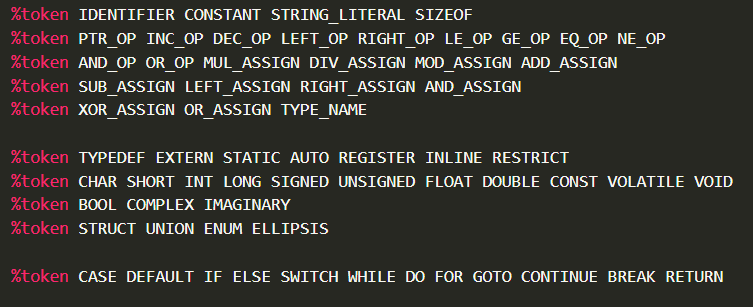
\includegraphics[width=.7\textwidth,keepaspectratio]{c99-ex2}
%     \caption{}
%     \label{token_c99}
% \end{figure}

Un'altra cosa che possiamo osservare è la dichiarazione di quello che è lo starting symbol della grammatica:
\ifthenelse{\boolean{isCompiledFromMain}}{%
\inputminted[firstline = 14, lastline = 14, linenos, breaklines, tabsize = 2]{c}{chapters/06/assets/resources/c99.y}%
}{%
\inputminted[firstline = 14, lastline = 14, linenos, breaklines, tabsize = 2]{c}{assets/resources/c99.y}%
}
Questa dichiarazione in realtà potrebbe non essere presente su alcuni file contenenti grammatiche, dal momento che, in sua assenza, non otteniamo degli errori, bensì viene preso il non-letterale della prima produzione listata a seguito come starting symbol.


Il ruolo dell’analizzatore lessicale è quindi analizzare il sorgente e decidere, di volta in volta, quale derivazione può essere applicata a ciascuna delle righe del sorgente analizzato. Una volta completato l'albero di derivazione e quindi arrivato presso un terminale (ad esempio \texttt{IDENTIFIER}), l'analizzatore lessicale andrà anche ad associargli informazioni come valore e tipo, dal momento che è necessario distinguere quell'\texttt{IDENTIFIER} da un altro. Nel programma potremmo appunto avere due \texttt{IDENTIFIER} di diverso tipo, ma in ogni caso dovremo conservare delle informazioni aggiuntive di qualche tipo (nome, tipo, scope e altro ancora). Tutte queste informazioni vengono conservate in una \emph{symbol table}.

Infine, le ultime righe del file contengono informazioni utili al particolare analizzatore sintattico utilizzato; avremo modo di parlarne nel dettaglio in futuro.

\subsection{Classi di tokens}
Si potrebbe a ragione considerare superfluo specificare che ogni diversa grammatica (e quindi ogni linguaggio) presenta diverse categorie di tokens; banalmente, il lettore è probabilmente ben cosciente che linguaggi diversi possiedono generalmente keyword diverse. Ad ogni modo, a seguito presentiamo alcune tra le scelte più ricorrenti:
\begin{itemize}
    \item un token per ogni keyword, quindi un token per ogni nome di base già presente nel linguaggio (\mintinline{c}{if}, \mintinline{c}{while}, \mintinline{c}{for} e via dicendo);
    \item un token per ogni operatore (o anche per classe di operatori), quindi in C ne avremo uno per \mintinline{c}{+} ma anche uno dedicato per \mintinline{c}{++}; 
    \item un unico token per gli identificatori, valido per tutti quanti;
    \item un token per ogni simbolo di punteggiatura. 
\end{itemize}

\subsection{Il compito dell'analizzatore lessicale}
L'obiettivo dell'analalizzatore lessicale è quindi riconoscere i cosiddetti \emph{lessemi}, ossia quelle parti del programma che corrispondono ai token, e ritornarli. Ciascuno di questi, di solito, viene ritornato sotto forma di coppia \texttt{<token-name>: <token-value>}, dove:
\begin{itemize}
    \item \texttt{<token-name>} è il nome scelto per denotare quel preciso token; seguendo l'esempio della grammatica precedente, \texttt{IDENTIFIER} è un \texttt{<token-name>};
    \item \texttt{<token-value>} è tipicamente un puntatore a una entry della symbol table, in cui si va a salvare tutte le informazioni relative a quel preciso token di tipo\footnote{In questo caso la parola "tipo" è chiaramente impropria, ma è molto utile per rendere la natura astratta di classe di token.} \texttt{<token-name>}.
\end{itemize}

\section{Lessemi e espressioni regolari}
Andiamo quindi a capire in che modo la teoria studiata nei due capitoli precedenti entra prepotentemente nell'analisi lessicale.

I lessemi sono estremamente facili da descrivere utilizzando le espressioni regolari: ad esempio, in un linguaggio che prevede un lessema identificatore, il quale è costituito di qualsiasi combinazione di lettere maiuscole e minuscole, quest'ultimo può essere facilmente denotato da un'espressione regolare del tipo:
\begin{equation*}
    (a \mid b \mid \ldots \mid z \mid A \mid B \mid \ldots \mid Z)^*
\end{equation*}
Questo è molto interessante: se è vero che i lessemi sono perfettamente descrivibili con dei linguaggi regolari, allora vuol dire che possiamo utilizzare quelli in sede di analisi lessicale, senza dover tirare in ballo i più potenti ma decisamente più complessi linguaggi liberi.

Quindi questi lessemi, essendo descritti da delle espressioni regolari, possono anche essere riconosciuti agevolmente da una macchina a stati finiti, come ad esempio quella in figura sotto, che descrive la classe \texttt{relop} di token per gli operatori relazionali.
\begin{figure}[H]
    \centering
    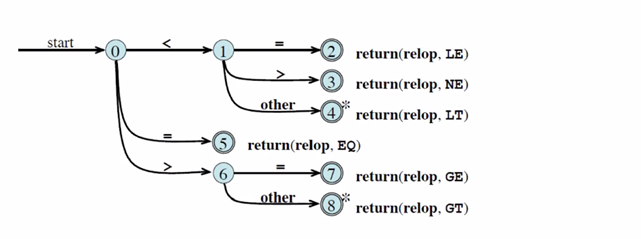
\includegraphics[width=\textwidth,keepaspectratio]{lec-14-1}
    \caption{}
    % \label{dfa-b_odd-and-a_even}
\end{figure}
È molto semplice intuire graficamente che ciascun percorso che termini in uno stato finale ritorna un token, sotto forma di coppia, in cui il \texttt{token-name} è appunto quello della classe \texttt{relop}, mentre il \texttt{token-value} indica qual è l'elemento della classe da ritornare.

\paragraph{Retract}
Possiamo notare che i due stati finali il cui arco entrante è marcato come \(other\) hanno anche un asterisco: questo indica che, quando consumo quella transizione, devo ricordarmi di tornare indietro di un simbolo, perché quest'ultimo simbolo \(other\) (cioè che non fa parte di alcun elemento appartenente alla classe \texttt{relop}) potrebbe essere un elemento di un token successivo, e se non facessimo quanto detto sopra rischieremmo di saltarla nell'analisi e ottenere un flusso di token incorretto. Questa operazione è detta \(retract\).

L'operazione di retract è uno dei tanti elementi legati alla gestione dell'input e del buffer che ci fanno pensare che la macchina a stati è un modello molto vicino al più noto, per noi, automa a stati finiti, ma quanto è profondo questo legame?

\subsection{Pattern matching basato su NFA}
Immaginiamo di avere delle espressioni regolari che denotano il linguaggio dei lessemi che siamo interessati a riconoscere. Si pensi ad esempio all'espressione regolare che denota il lessema \texttt{IDENTIFIER}, ossia l'espressione regolare che denota tutte le possibili combinazioni di lettere maiuscole e minuscole (con le dovute peculiarità di ciascun linguaggio); oppure, si pensi a un'espressione regolare che denoti il lessema degli operatori relazionali, o ancora un'altra che denoti la scrittura dei floating numbers. In sostanza, per ciascuna categoria sintattica abbiamo un'espressione regolare che la denota.

Sappiamo anche che, avendo delle espressioni regolari, per ciascuna di queste possiamo costruire un NFA che riconosce il linguaggio denotato dall'espressione considerata; possiamo a questo punto immaginare di far collidere questi NFA inserendo uno stato iniziale extra e collegandolo a ciascun NFA tramite una \(\varepsilon\)-transizione, come mostrato in Fig.\ref{nfa_for_grammar_regular_expressions} sotto.
Da notare che nel caso d'uso del compilatore ci sono delle azioni associate agli stati finali (se l'analizzatore legge un assegnamento compie, appunto, le azioni per registrare l'assegnamento).
\begin{figure}[H]
    \centering
    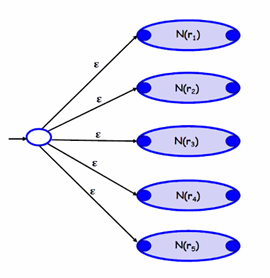
\includegraphics[width=.4\textwidth,keepaspectratio]{lec-14-2}
    \caption{}
    \label{nfa_for_grammar_regular_expressions}
\end{figure}
Una struttura di questo tipo può riconoscere i linguaggi denotati da tutte le espressioni regolari per cui abbiamo costruito degli NFA. 

Adesso dobbiamo pensare come ottimizzare l'uso di una struttura simile per l'analisi lessicale. Potremmo trovarci infatti a gestire problemi di diversa natura, in particolare relativi all'input buffering: ad esempio, come posso fare a sapere se i due caratteri \texttt{i} e \texttt{f} che ho appena letto stanno a indicare la keyword \mintinline{c}{if} e non un ipotetico identificatore \mintinline{c}{iffoff}? Detto in maniera informale, come decido quando fermarmi, quando tornare indietro, quando e se ho letto più di quanto mi serviva?

Il procedimento che seguiamo è il seguente:
\begin{enumerate}
    \item innanzitutto simuliamo l'NFA creato come sopra descritto;
    \item nel caso di ambiguità, ossia di situazioni come quella descritta sopra tra \mintinline{c}{if} e \mintinline{c}{iffoff}, la convenzione è di preoseguire la simulazione finché nessun’altra transizione è possibile, solitamente quando incontriamo uno spazio o un \texttt{\(\backslash\)n}, privilegiando quindi il match più lungo (si parla di cercare il \emph{longest match});
    \item se nell'insieme di stati che abbiamo raggiunto ci sono delle azioni disponibili, allora andremo ad eseguire quella appartenente al longest match, in caso di pareggio ciascuna azione avrà una priorità, e noi eseguiremo quella con più alta priorità;
    \item se nessun'azione è disponibile, dobbiamo invece tornare indietro nella sequenza di stati percorsi, fermarci nel primo insieme di stati che presenta almeno uno stato finale e delle azioni associate e cercare di nuovo quella prioritaria; per ognuno di questi passi all'indietro, dobbiamo ricordari di aggiornare il puntatore all'input buffer.
\end{enumerate}

Tutto questo funzionerebbe in maniera analoga se utilizzassimo un DFA: dovremmo semplicemente costruire il DFA a partire dal NFA, dimodoché l'insieme degli stati del DFA sia un sottoinsieme di quello dell'NFA corrispondente.

\subsection{Generatori di analizzatori lessicali: Flex}
Andiamo a parlare quindi di questi generatori. L'idea di creare un generatore di analizzatori lessicali è nata in concomitanza con la prima definizione e implementazione del compilatore del C, e l'idea era di evitare di dover scrivere ogni volta, per ogni programma, un analizzatore lessicale e uno sintattico a mano.

\emph{Flex} è il primo della sua specie\footnote{o meglio, una sua versione più moderna: il primo vero e proprio si chiamava \emph{lex} e quella \emph{f}, aggiunta successivamente, sta per fast.} ed è solitamente compreso nelle distribuzioni di C; l'idea è risultata talmente valida che oggigiorno ogni linguaggio possiede un proprio generatore di analizzatore lessiale e sintattico.

Il funzionamento di Flex (ma anche di tutti i generatori di questo tipo) è il seguente: 
\begin{itemize}
    \item andremo a creare un file del tipo \texttt{file.l}, il quale sarà l'input del generatore e in cui scriveremo quali sono i pattern che vogliamo riconoscere e quali sono le azioni da compiere in corrispondenza dei vari matches;
    \item a quel punto, possiamo compilare \texttt{file.l} utilizzando il comando \texttt{Flex}, e questo ci restituirà un file di nome \texttt{lex.yy.c}\footnote{La ragione di questo nome è puramente convenzionale e deriva dal fatto che, storicamente, il generatore Flex è stato usato in coppia all'analizzatore \emph{Yacc}};
    \item compilando questo \texttt{lex.yy.c} con il compilatore \texttt{gcc} otteniamo il \emph{lexer}, cioè quel signore che si occupa di gestire l'input buffering, di fare le operazioni di retract e altro ancora.
\end{itemize} 
\begin{minted}[breaklines, tabsize = 2]{bash}
    $   Flex file.l
    $   gcc lex.yy.c -lfl
    $   ./a
\end{minted}
Si tenga bene a mente che queste tre righe descrivono come utilizzare Flex da solo; tuttavia, quest'ultima è un'eventualità piuttosto rara, dal momento che Flex è nato per essere usato in pipeline con un generatore di analizzatore di analisi sintattica, ma poiché questi sono elementi ancora sconosciuti per noi, al momento non ce ne preoccupiamo.

\subsection{Struttura del \texttt{file.l}}
I file con estensione \texttt{.l} che diamo da fagocitare a Flex hanno la seguente struttura:
\begin{minted}[breaklines, tabsize = 2]{bash}
...
//(Preambolo)
% { code
% }
// shorthand for patterns
%%
//(Parte centrale)
pattern-1 {action-1};
pattern-2 {action-2};
...
%%
//(Epilogo)
user routines
\end{minted}
Il contenuto di queste tre macrosezioni è ben determinato, andiamo a vederlo più da vicino:
\begin{labeling}{Parte centrale}
    \item[Preambolo] qui ci andrà del codice C,in particolare le inizializzazioni di variabili, o delle abbreviazioni per indicare dei particolari pattern nelle espressioni regolari che andremo a utilizzare sotto;
    \item[Parte centrale] è il cuore del file, e si tratta di una lista pattern-azione, dove pattern è un'espressione regolare, e l'azione sarà ciò che dobbiamo compiere qualora dovessimo riconoscere il pattern corrispondente;
    \item[Epilogo] questa sezione è in realtà facoltativa, il lexer funziona anche senza che vi sia scritto alcunché; tuttavia, quello che potremmo eventualmente trovare e/o scrivere qui dentro sono delle routine definite dall'utente, le quali verranno copiate e incollate dentro al genituro \texttt{lex.yy.c}.
\end{labeling}

\subsection{Il linguaggio delle espressioni regolari in Flex}
Dal momento che tutte le coppie \texttt{pattern \{azione\}} sono scritte in linguaggio \texttt{lex}, a differenza di altre parti di \texttt{file.l}, è opportuno conoscere questo linguaggio. Di seguito presentiamo i \emph{metacaratteri} di Flex, ossia dei caratteri riservati:
\begin{equation*}
    \slash \quad \backslash \quad - \quad * \quad + \quad >\quad " \quad \{ \quad \} \quad . \quad \$ \quad ( \quad ) \quad \mid \quad \% \quad [ \quad ] \quad ^\wedge
\end{equation*}
\noindent Andiamo a vedere più da vicino quali sono le regole di matching dei metacaratteri:
\begin{labeling}{a | b}
    \item[\texttt{.}] qualsiasi carattere, eccetto il newline;
    \item[\texttt{\(\backslash\)n}] il newline;
    \item[\texttt{*}] zero o più copie di un elemento;
    \item[\texttt{+}] una o più copie di un elemento;
    \item[\texttt{?}] zero o una copia di un elemento;
    \item[\texttt{[]}] denota le classi di caratteri: al posto di \(a \mid b \mid \ldots \mid z\), posso scrivere \texttt{[a-z]};
    \item[\texttt{\(^\wedge\)}] inizio di riga, negazione se usato in una classe di caratteri;
    \item[\texttt{\$}] end of line;
    \item[\texttt{a|b}] pipe, semantica consueta  (i.e. a or b);
    \item[\texttt{()}] raggruppamenti;
    \item[\texttt{"+"}] il literal \texttt{"+"} (è necessario usare qusto metodo di escape per poter far riferimento ad un carattere qualunque e non al metacarattere)
    \item[\texttt{\{\}}] espressioni regolari scritte nel preambolo
\end{labeling}


\section{Esempi di file per Flex}
Facciamo un breve riepilogo di quanto abbiamo visto: tutti i file predisposti per Flex si compongono di  tre sezioni, ciascuna separata da coppie di \%. Nel preambolo si inseriscono delle definizioni come le \mintinline{c}{define} che servono e i pattern (espressioni regolari per i lessemi che vogliamo inserire). I pattern sono inseriti insieme all'azione nella parte centrale. In fondo si inseriscono le routine dell'utente che vengono copiate nel file \texttt{lex.yy.c}: un testo minimale è l'invocazione della routine \mintinline{c}{yylex()} che se non viene inserita viene chiamata in automatico. I comandi, qualora non si usi Flex con Bison (analizzatore sintattico in pipeline con Flex), sono i seguenti:
\begin{minted}[breaklines, tabsize = 2]{bash}
    $   Flex file.l
    $   gcc lex.yy.c -lfl
    $   ./a
\end{minted}

\subsection*{file0.l}
\ifthenelse{\boolean{isCompiledFromMain}}{%
\inputminted[linenos, breaklines, tabsize = 2]{c}{chapters/06/assets/code-fragments/file0.l}%
}{%
\inputminted[linenos, breaklines, tabsize = 2]{c}{assets/code-fragments/file0.l}%
}
% \begin{figure}[h]
%     \centering
%     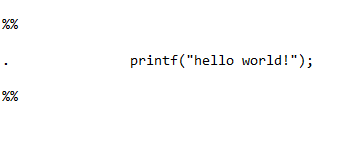
\includegraphics[width=.7\textwidth,keepaspectratio]{file0.l.png}
%     \caption{file0.l}
%     \label{file0.l}
% \end{figure}

In qusto primo esempio vediamo che nel preambolo non sono presenti né delle \texttt{define} né del codice; dal momento che non sono presenti routine inserite dall'utente, verrà invocata la procedura \texttt{yylex()} all'esecuzione. Basandoci sulla sintassi di Flex vista precedentemente, andiamo ad analizzare la parte centrale costituita da una sola coppia pattern-azione:
\begin{itemize}
    \item il pattern è dato dalla regular expression composta solo da \texttt{.}, il che significa che l'azione seguente farà riferimento a tutti i caratteri incontrati, tranne quello di \texttt{\(\backslash\)n} (\emph{new line});
    \item l'azione è quel \mintinline{c}{printf("hello world!")}, il che consiste banalmente nello stampare la stringa hello world ogni volta che viene eseguito un match sul pattern.
\end{itemize}
In sostanza, questo file ci farà sì che, nella lettura, qualsiasi carattere incontriamo, ad eccezione del new line, verrà sostituito da un'occorrenza della stringa \texttt{"hello world!"}; quindi, ad esempio:
\begin{itemize}
    \item \(a\) diventerà \texttt{hello world!};
    \item \(aa\) diventerà \texttt{hello world!hello world!}.
\end{itemize}

Possiamo notare anche un'altra cosa molto interessante: solitamente, per poter utilizzare lo standard output nei programmi C, è necessario includere all'interno del file la libreria \mintinline{c}{stdio.h}, ma nel \texttt{file0.l} non vi è nemmeno l'ombra di un inlcude: è lo stesso Flex a occuparsi di aggiungere in un secondo momento tutti i dettagli necessari per la gestione dell'output.

\subsection*{file1.l}
\ifthenelse{\boolean{isCompiledFromMain}}{%
\inputminted[linenos, breaklines, tabsize = 2]{c}{chapters/06/assets/code-fragments/file1.l}%
}{%
\inputminted[linenos, breaklines, tabsize = 2]{c}{assets/code-fragments/file1.l}%
}

% \begin{figure}[h]
%     \centering
%     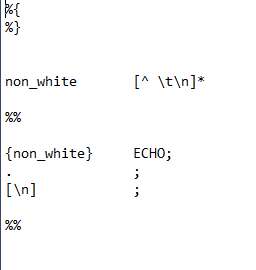
\includegraphics[width=.7\textwidth,keepaspectratio]{file1.l.png}
%     \caption{file1.l}
%     \label{file1.l}
% \end{figure}

\paragraph{Preambolo}
Diversamente dall'esempio precedente, in questo \texttt{file1.l} abbiamo del contenuto nel preambolo. Andiamo a vederlo nel dettaglio:

\begin{enumerate}
    \item il primo blocco (righe 1 e 2, in questo caso vuoto) è identificato dal simbolo di apertura \texttt{\%\{} e cui può seguire del codice C;
    \item il secondo blocco (righe da 3 a 6), invece, è successivo al simbolo di chiusura \texttt{\%\}} e contiene quelli che sono gli shorthands per i pattern, vale a dire degli alias per delle espressioni regolari.
\end{enumerate}

Rifacendoci sempre alla sintassi di Flex, possiamo analizzare l'espressione regolare definita nel preambolo e arrivare alla conclusione che faccia riferimento a quell'insieme di caratteri (\texttt{[ ]}) che si ripetono \(0\) o più volte (*) e che sono diversi (\^{}) da '\texttt{ }', '\texttt{\textbackslash t}' e '\texttt{\textbackslash n}'; questo significa che comporteranno un match tutte quelle sequenze di caratteri che sono separate da spazi, tab o new line; più semplicemente, saranno le parole a causare un match.

\paragraph{Parte centrale}
Come descritto precedentemente, nella parte centrale i pattern sono associati alle relative azioni; in questo caso, le coppie che troviamo sono le seguenti:
\begin{itemize}
    \item \texttt{non\_white} comporta l'esecuzione della macro \mintinline{c}{echo} di Flex, che è equivalente a \mintinline{c}{printf("\%s", yytext)} in linguaggio C, e stamperà a video esattamente la sequenza di caratteri che ha causato il match;
    \item un qualunque carattere diverso da \texttt{\textbackslash n (.)} verrà eliminato;
    \item new line (\texttt{\textbackslash n}) verrà anch'esso eliminato
\end{itemize}

Complessivamente, il risultato ottenuto dall'esecuzione di un programma compilato a partire dal file discusso porterà all'eliminazione di '\texttt{ }', '\texttt{\textbackslash t}' e '\texttt{\textbackslash n}' dal testo passato in input e ci farà ottenere ad una sequenza continua di caratteri (ad esempio, una stringa del tipo "\texttt{ ab c d e \hspace{.8cm} f g}" diventerà "\texttt{abcdefg}").

\subsection*{file2.l}

\ifthenelse{\boolean{isCompiledFromMain}}{%
\inputminted[linenos, breaklines, tabsize = 2]{c}{chapters/06/assets/code-fragments/file2.l}%
}{%
\inputminted[linenos, breaklines, tabsize = 2]{c}{assets/code-fragments/file2.l}%
}

% \begin{figure}[h]
%     \centering
%     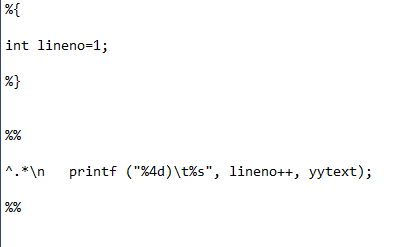
\includegraphics[width=.7\textwidth,keepaspectratio]{file2.l.png}
%     \caption{file2.l}
%     \label{file2.l}
% \end{figure}

\paragraph{Preambolo}
In questo esempio, invece, troviamo finalmente del codice C nel preambolo; in particolare, troviamo la dichiarazione di un intero chiamato \texttt{lineno} ed inizializzato al valore \(1\). 

\paragraph{Parte centrale}
A seguire abbiamo la parte centrale del file, dove: 

\begin{itemize}
    \item all'espressione regolare \texttt{\^{}.*\textbackslash n}, che identifica tutte quelle sequenze di caratteri che iniziano per un carattere differente da new line ripetuto zero o più volte e finiscono per new line o, più semplicemente, le parole sulla stessa riga
    \item  viene associata l'azione \mintinline{c}{printf("\%4d)\t\%s", lineno++, yytext)}, che stampa il valore dell'intero lineno seguito dal simbolo ) e dal contenuto del buffer \mintinline{c}{yytext} (che contiene l'input fino ad ora riconosciuto) ed infine esegue il postincremento di lineno.
\end{itemize}

\noindent Quindi, il nostro programma si occuperà di stampare tutte le parole sulla stessa riga anteponendo il numero della riga a cui fa riferimento; in altre parole, se avessimo un testo come il seguente:
\begin{itemize}[noitemsep]
    \item[] \emph{Autem quo ea. Voluptatum saepe porro. Quibusdam illo eum.}
    \item[] \emph{Quia aperiam nesciunt. Qui est voluptate. Aut temporibus perspiciatis.}
    \item[] \emph{Repudiandae delectus omnis. Modi earum doloribus. Quis eaque quidem.}
\end{itemize}
Allora otterremmo in output:
\begin{enumerate}[noitemsep]
    \item[\texttt{1}] \emph{Autem quo ea. Voluptatum saepe porro. Quibusdam illo eum.}
    \item[\texttt{2}] \emph{Quia aperiam nesciunt. Qui est voluptate. Aut temporibus perspiciatis.}
    \item[\texttt{3}] \emph{Repudiandae delectus omnis. Modi earum doloribus. Quis eaque quidem.}
\end{enumerate}


\subsection*{file3.l}
\ifthenelse{\boolean{isCompiledFromMain}}{%
\inputminted[linenos, breaklines, tabsize = 2, fontsize = \small]{c}{chapters/06/assets/code-fragments/file3.l}%
}{%
\inputminted[linenos, breaklines, tabsize = 2, fontsize = \small]{c}{assets/code-fragments/file3.l}%
}

% \begin{figure}[h]
%     \centering
%     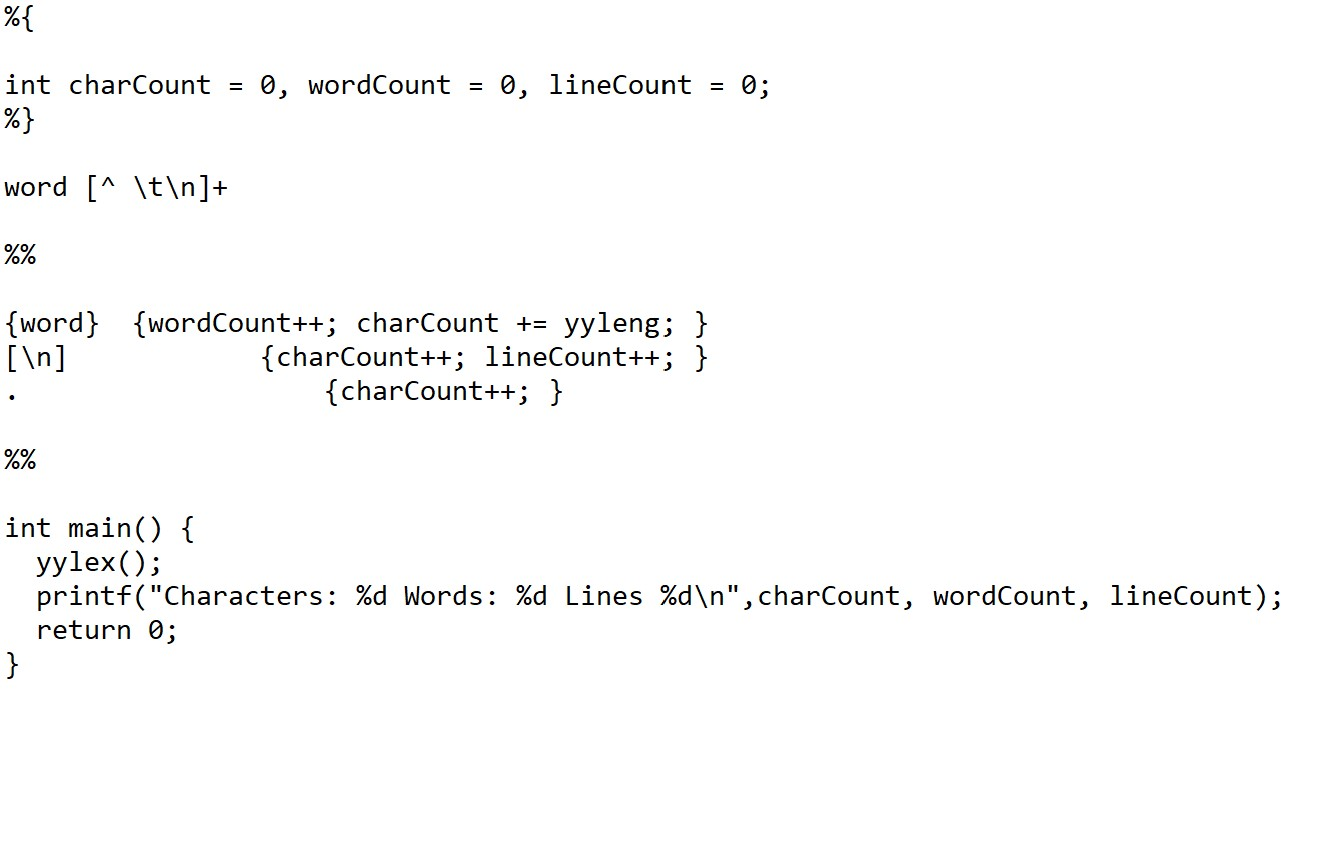
\includegraphics[width=.7\textwidth,keepaspectratio]{file3.l.jpg}
%     \caption{file3.l}
%     \label{file3.l}
% \end{figure}

In questo quarto esercizio andiamo a combinare quanto visto precedentemente, aggiungendo anche una routine custom scrivendo del codice ad hoc nell'epilogo del file.

\paragraph{Preambolo}
Nel preambolo abbiamo la dichiarazione di tre variabili che ci serviranno nelle routine come contatori; inoltre, abbiamo anche una shorthand, chiamata \texttt{word}, la cui espressione regolare include tutte quelle sequenze di uno o più caratteri (\texttt{+}) che non contengono '\texttt{ }', '\texttt{\textbackslash t}' e '\texttt{\textbackslash n}.

\paragraph{Parte centrale}
Nella parte centrale del file abbiamo invece le seguenti associazioni pattern-azione:

\begin{itemize}
    \item \texttt{word} comporta l'esecuzione del seguente pezzo di codice \texttt{\{wordCount++; charCount += yyleng; \}}, dove la variabile \texttt{wordCount} viene postincrementata, mentre alla variabile \texttt{charCount} viene sommato un numero pari a \texttt{yyleng}, che contiene la lunghezza della stringa riconosciuta e, per via dell'espressione regolare alla base della shorthand, equivalente a quella della parola;
    \item il secondo pattern è \texttt{\textbackslash n}, cioè nel caso in cui si trovi una sequenza di caratteri composta solamente da una new line; l'azione legata è il blocco \mintinline{c}{{charCount++; lineCount++; }}, dove si postincrementano sia \mintinline{c}{charCount} che \mintinline{c}{lineCount};
    \item infine, l'ultimo pattern, il punto (\texttt{.}), comporta solamente il postincremento della variabile \mintinline{c}{charCount}.
\end{itemize}

In sostanza, il programma che stiamo descrivendo con questi pattern si occupa di contare complessivamente quanti caratteri, parole e righe sono state individuate in un dato testo; qualora avessimo un match con una parola, allora avviene un incremento proporzionale al numero di caratteri che costituiscono quella stessa parola e, inoltre, si aggiorna il numero di parole totali che sono contenute nel testo; ogni volta che si trova una new line si incrementano di un'unità il numero di righe e di caratteri e, infine, ogni volta che si trova uno spazio o un tab viene incrementato solamente il numero di caratteri. 

\subsection*{file4.l} 
\ifthenelse{\boolean{isCompiledFromMain}}{%
\inputminted[linenos, breaklines, tabsize = 2, fontsize = \small]{c}{chapters/06/assets/code-fragments/file4.l}%
}{%
\inputminted[linenos, breaklines, tabsize = 2, fontsize = \small]{c}{assets/code-fragments/file4.l}%
}
\noindent L'ultimo esempio proposto fa uso di quanto discusso fino ad ora per analizzare un \texttt{csv} e restituire i dati sotto forma di una tabella in formato \texttt{html}; inoltre, potremo osservare un'implementazione del longest match.

\paragraph{Preambolo}
Nel preambolo viene dichiarata una variabile intera \mintinline{c}{comma}, che è inizializzata a \(0\); servirà per controllare le entry vuote nel \texttt{csv} passato in input date da virgole consecutive.

\paragraph{Parte centrale}
Andiamo a vedere da vicino le coppie pattern-azione che troviamo nella parte centrale.
\begin{itemize}
    \item L'espressione regolare \mintinline{c}{[a-zA-Z0-9]+}, che indica la sequenza di uno o più caratteri alfanumerici, comporta l'esecuzione di \texttt{printf("<td>"); ECHO; comma = 0;}, dove viene creata una nuova colonna per la tabella, viene inserita la sequenza appena letta e viene impostato il valore dell'intero \mintinline{c}{comma} a \(0\).
    \item La seconda espressione è "\texttt{,}", che vuol dire che bisogna trovare il carattere che corrisponde alla virgola e che nel \texttt{csv} serve per separare i dati, comporta l'esecuzione del blocco di codice
    \begin{minted}[breaklines, tabsize = 2]{c}
    {            
    if (comma) {
        printf("<td> </td>"); 
    } else { 
        printf("</td>");
    }       
        comma = 1;
    }
    \end{minted}
        
    dove viene verificato il numero di virgole incontrate fino a quel punto: se si sono incontrate 0 virgole, allora si chiude semplicemente la colonna precedentemente aperta; se invece si è già incontrata \(1\) virgola e, consecutivamente, se ne legge un'altra (o comunque le due occorrenze risultano essere separate da sequenze non alfanumeriche), viene creata una colonna vuota, in quanto nel \texttt{csv} non vi sono dati rilevanti. In ogni caso alla fine del blocco viene impostato il valore di comma ad \(1\).
    \item In ultimo, \texttt{\textbackslash n}, cioè per ogni new line viene eseguito il blocco di codice \mintinline{c}{{printf("</tr> \n <tr>"); comma = 0;}} dove viene chiusa la riga precedente ed aperta quella successiva.
\end{itemize}

\paragraph{Epilogo}
Nell'epilogo troviamo una routine custom dove viene creato l'html di base per creare la tabella e, tra le varie cose, viene anche aperta la prima riga. Dopo aver stampato lo scheletro della struttura viene invocata la procedura \mintinline{c}{yylex()}, la quale cerca i pattern nel testo; infine, la tabella viene chiusa.

\subsection{Ulteriori informazioni su Flex}
Quando abbiamo discusso del funzionamento dell'analisi lessicale basata sull'utilizzo di NFA o DFA abbiamo anche parlato del fatto che, quando si tenta di riconoscere il pattern di una determinata parola, è possibile che avvengano dei match su più stati finali dell'automa e che quindi si possa avere il dubbio su quale azione eseguire: come si riflette tutto ciò in Flex? 

Per risolvere a tale problematica si utilizza la regola del \emph{longest match}: dalla lista di pattern si va a recuperare quello più lungo che ha portato ad un match.

Cosa succede invece se ci sono più pattern che a parità di lunghezza comportano un match (ovvero i due pattern hanno la stessa lunghezza)? In questo caso si sceglie sempre il primo della lista. Da qui si intuisce dunque che anche l'ordine in cui si scrive la sequenza dei pattern ha una sua importanza: un medesimo \texttt{file.l} potrebbe non generare lo stesso risultato se si eseguisse uno shuffle dei pattern.

\end{document}